
\documentclass[11pt,a4paper,onecolumn,openright,oneside]{report}
\usepackage[utf8]{inputenc}
\usepackage[utf8]{inputenc}
\usepackage[T1]{fontenc}
\usepackage[top=2cm, bottom=2cm]{geometry}
\usepackage{float}%positionner les images
\usepackage{graphicx}%pour les images
\usepackage{soul}

\usepackage[french]{babel}
\usepackage{parselines} 

\graphicspath{ {./images/} }%specifier le dossier ou se trouve les images 


\newcommand{\HRule}{\rule{\linewidth}{0.5mm}} %------- Faire les trai Dans La Page De Garde

\usepackage{mathtools}%equation mathematique qui depasse le cadre
\usepackage{indentfirst} %indentation
\usepackage{fullpage}
\usepackage{color}
\usepackage[table]{xcolor}

 
\definecolor{darkWhite}{rgb}{0.94,0.94,0.94}
\usepackage{listings} %ecriture de partie code scilab ou autre dans latex
\lstset{
  aboveskip=3mm,
  belowskip=-2mm,
  backgroundcolor=\color{darkWhite},
  basicstyle=\footnotesize,
  breakatwhitespace=false,
  breaklines=true,
  captionpos=b,
  commentstyle=\color{red},
  deletekeywords={...},
  escapeinside={\%*}{*)},
  extendedchars=true,
  framexleftmargin=16pt,
  framextopmargin=3pt,
  framexbottommargin=6pt,
  frame=tb,
  keepspaces=true,
  keywordstyle=\color{blue},
  language=C,
  literate=
  {²}{{\textsuperscript{2}}}1
  {⁴}{{\textsuperscript{4}}}1
  {⁶}{{\textsuperscript{6}}}1
  {⁸}{{\textsuperscript{8}}}1
  {€}{{\euro{}}}1
  {é}{{\'e}}1
  {è}{{\`{e}}}1
  {ê}{{\^{e}}}1
  {ë}{{\¨{e}}}1
  {É}{{\'{E}}}1
  {Ê}{{\^{E}}}1
  {û}{{\^{u}}}1
  {ù}{{\`{u}}}1
  {â}{{\^{a}}}1
  {à}{{\`{a}}}1
  {á}{{\'{a}}}1
  {ã}{{\~{a}}}1
  {Á}{{\'{A}}}1
  {Â}{{\^{A}}}1
  {Ã}{{\~{A}}}1
  {ç}{{\c{c}}}1
  {Ç}{{\c{C}}}1
  {õ}{{\~{o}}}1
  {ó}{{\'{o}}}1
  {ô}{{\^{o}}}1
  {Õ}{{\~{O}}}1
  {Ó}{{\'{O}}}1
  {Ô}{{\^{O}}}1
  {î}{{\^{i}}}1
  {Î}{{\^{I}}}1
  {í}{{\'{i}}}1
  {Í}{{\~{Í}}}1,
  morekeywords={*,...},
  numbers=left,
  numbersep=10pt,
  numberstyle=\tiny\color{black},
  rulecolor=\color{black},
  showspaces=false,
  showstringspaces=false,
  showtabs=false,
  stepnumber=1,
  stringstyle=\color{gray},
  tabsize=4,
  title=\lstname,
}
 



\usepackage{listing}

\usepackage{url}
\makeatletter
\renewcommand*{\thesection}{\arabic{section}}
\usepackage{booktabs}

\makeatother

\begin{document}


\section{Nbody2D}
\textbf{Makefile}\\

Comme on peut le voir sur le Makefile suivant, notre programme est compilé sans aucune optimisation afin de commencer notre analyse depuis le début.
\begin{figure}[H]
    \centering
    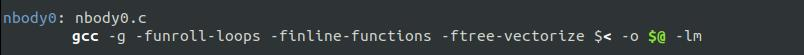
\includegraphics[scale=0.55]{Images/1/makefile.jpg}
    \caption{Makefile}
    \label{fig:my_label}
\end{figure}

\subsection{Sortie de Maqao}

Une fois MAQAO lancer avec les flags de base lui permettant à faire son analyse. On a des fichier htmls en sortie on exploite alors les informations mises a disposition afin d'optimiser notre programme : 
\begin{figure}[H]
    \centering
    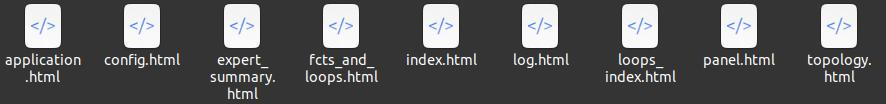
\includegraphics[scale=0.5]{Images/1/maqao.jpg}
    \caption{Sortie de l'execution de MAQAO}
    \label{fig:my_label}
\end{figure}

\subsubsection{1.1.1 Index}
On commence notre analyse par la page d'accueil du rapport. Sur cette page, on retrouve les informations sur le temps d'execution et si il est possible d'optimiser notre programme ou pas et les infos relative a la machine d'execution de programme.

\begin{figure}[H]
    \centering
    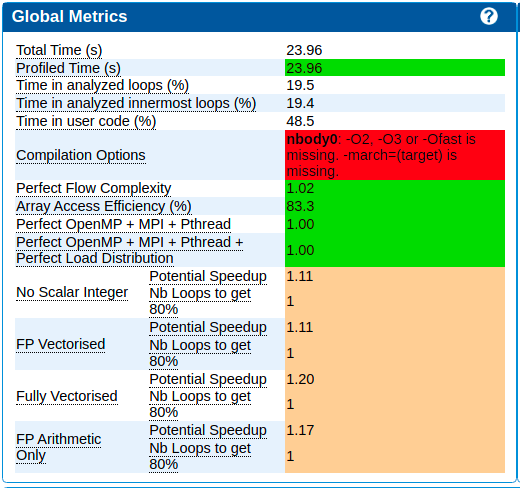
\includegraphics[scale=0.45]{Images/1/Global-Metric.png}
    \caption{Global Metrics}
    \label{fig:my_label}
\end{figure}

En observant les métriques globales du binaire analysé, on constate que celui-ci a été compilé sans flags d'optimisation ni de flags de spécification
d'architecture. De plus, on voit que d'une part, nos accès mémoire sont efficaces à 83.3\% (la valeur est bonne mais pourrait être amélioré) et des speed-up
peuvent-être otbtenus si le programme est vectorisé à la compilation.\\

A cette étape, nous allons prendre en compte la suggestion des flags -O2, -O3 or -Ofast, -march=(target) et pour le prochain binaire à produire.

\subsubsection{1.1.2 Experiment Summary}
\begin{figure}[H]
    \centering
    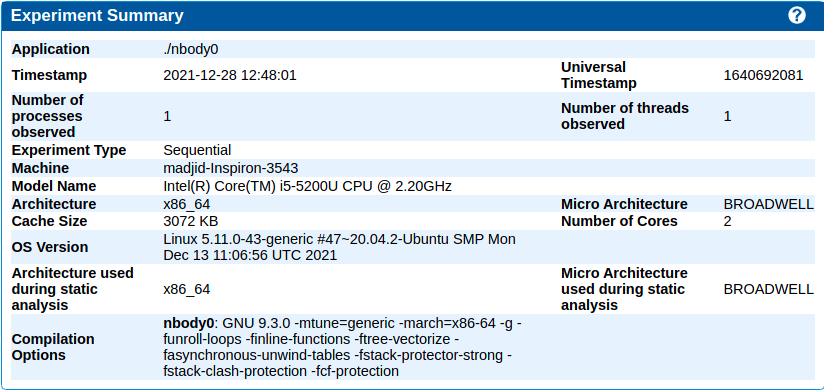
\includegraphics[scale=0.4]{Images/1/Experiment-Summary.png}
    \caption{Experiment-Summary}
    \label{fig:my_label}
\end{figure}
Experiment Summary nous donne les informations lien à la machine d'execution et ce que le compilateur a ajouter a notre place.

\subsection{Application}

La partie application nous donne des détails sur comment le temps a etait passé entre plusieurs categories (System, Binary, Math, IO etc..) et ou notre application passe beaucoup de temps.

\begin{figure}[H]
    \centering
    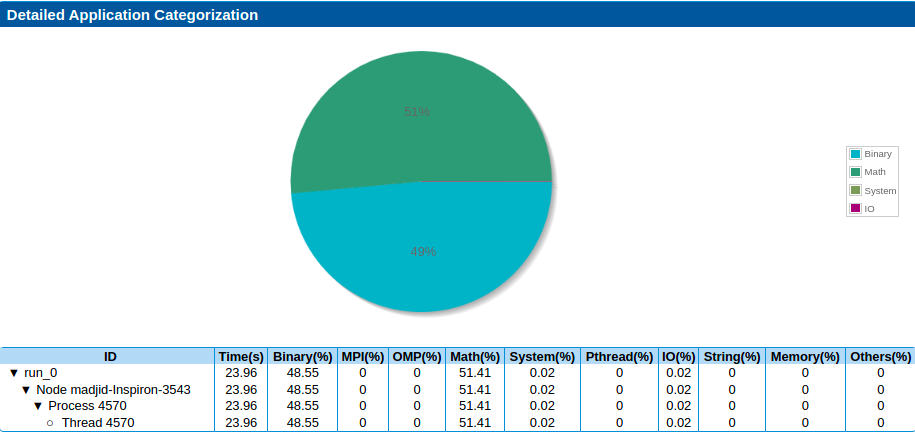
\includegraphics[scale=0.4]{Images/1/Application.png}
    \caption{Applications}
    \label{fig:my_label}
\end{figure}
Dans notre cas notre programme passe 51.41\% de son temps dans les methodes mathématiques et 48.55\% dans binary(code utilisateur).

\subsection{Loops}
Ici dans cette section on retrouve toutes les boucles qui prennes de temps a s'éxecuter par ordre et les détails sur la convergence la vectorizations etc...
\begin{figure}[H]
    \centering
    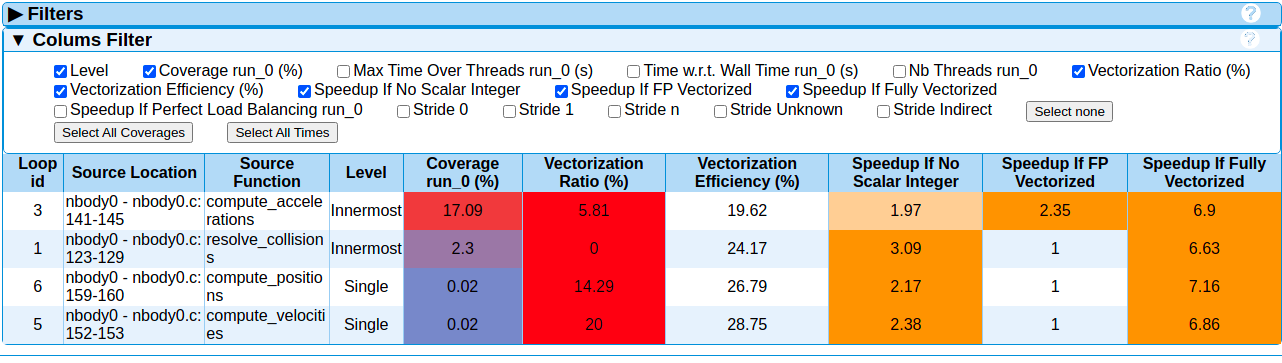
\includegraphics[scale=0.37]{Images/1/loops.png}
    \caption{Loops}
    \label{fig:my_label}
\end{figure}

On remarque  qu'une boucle à une couverture de 17\% on cliquant sur elle on affiche son rapport \textbf{CQA}.

\subsubsection{1.3.1 Rapport CQA}
Le rapport CQA il nous indique quelle boue de boucle consomme le plus et se présente comme la montre la figure suivante :
\begin{figure}[H]
    \centering
    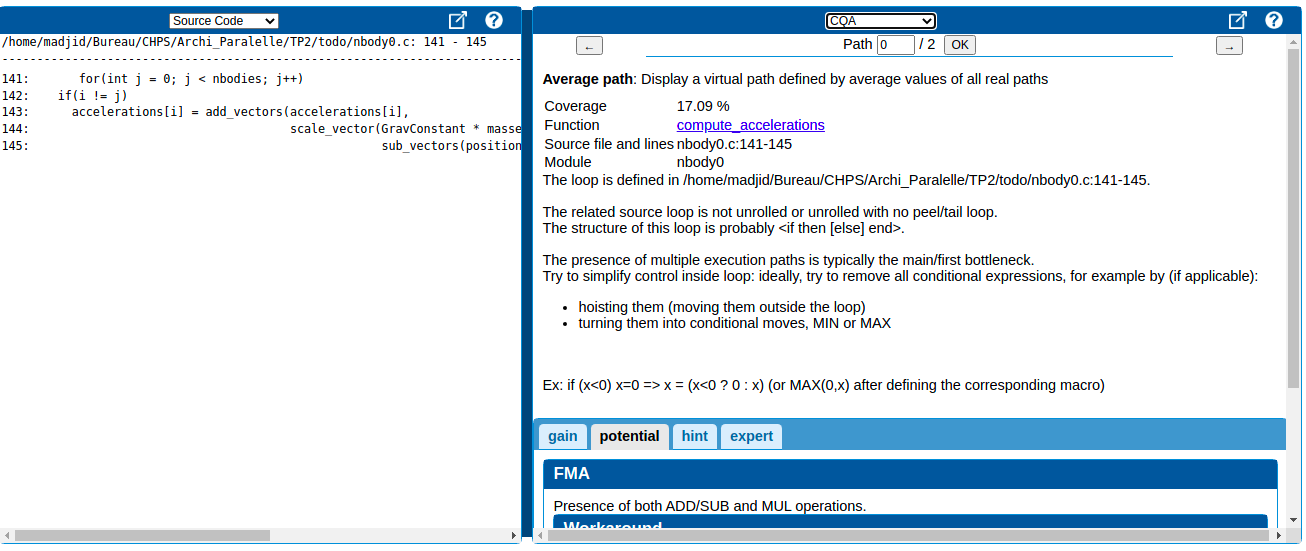
\includegraphics[scale=0.37]{Images/1/CQA.png}
    \caption{Rapport CQA}
    \label{fig:my_label}
\end{figure}
\newpage
\subsubsection{Détails de rapport CQA}
\textbf{Gain}\\

Dans cette partie MAQAO nous fais une estimations de gain de temps on vectorisant notre boucle et on donnant solution de contournement en changent la structure de Arrays of Structure (AoS) à Structure of Arrays (SoA).
\begin{figure}[H]
    \centering
    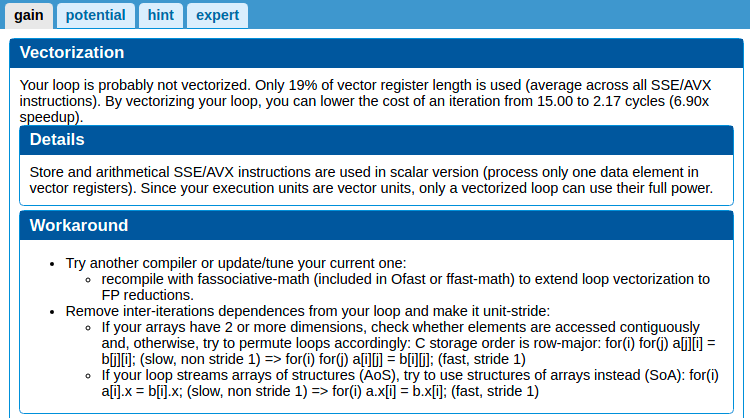
\includegraphics[scale=0.5]{Images/1/gain.png}
    \caption{Gain}
    \label{fig:my_label}
\end{figure}
\textbf{Potential}\\

MAQAO nous recommande de recompilé avec march=broadwell vu que il a detecter notre architecture est nous proposes la meilleur target possible.\\

MAQAO détecter aussi la présence d'ADD/SUB et MUL et il nous recommande de changer de synthaxe et passé de a + b*c est un FMA valide (MUL puis ADD). Cependant (a+b)* c ne peut pas être traduit en FMA (ADD puis MUL).
\begin{figure}[H]
    \centering
    \includegraphics[scale=0.5]{Images/1/potential.png}
    \caption{potential}
    \label{fig:my_label}
\end{figure}
\newpage

\textbf{Hint}\\

Dans cette partie MAQAO nous fais la  correspondance entre nous differentes boucles (dans le code source) et la boucle binaire dans notre cas ils nous donne combien d'opérations arithmétiques notre boucle éxecute.
\begin{figure}[H]
    \centering
    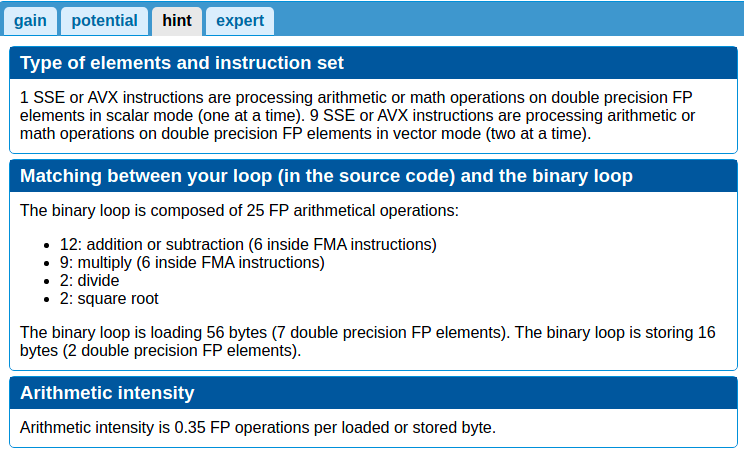
\includegraphics[scale=0.5]{Images/1/Hint.png}
    \caption{Hint}
    \label{fig:my_label}
\end{figure}

\section{Optimiser}
\subsection*{Makefile}
Cette fois on prend on compte les suggestion de MAQAO on changent la ligne de compilation on ajoutant -Ofast -funroll-loops -march=broadwell.
\begin{figure}[H]
    \centering
    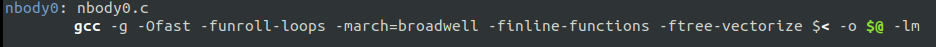
\includegraphics[scale=0.5]{Images/2/makefile.png}
    \caption{Makefile modifier}
    \label{fig:my_label}
\end{figure}

\subsection{Global Metrics }
Maintenant on remaque que on changent la compilation de Makefile on a ganger on temps et on vectorization et toutes est devenu verts.
\begin{figure}[H]
    \centering
    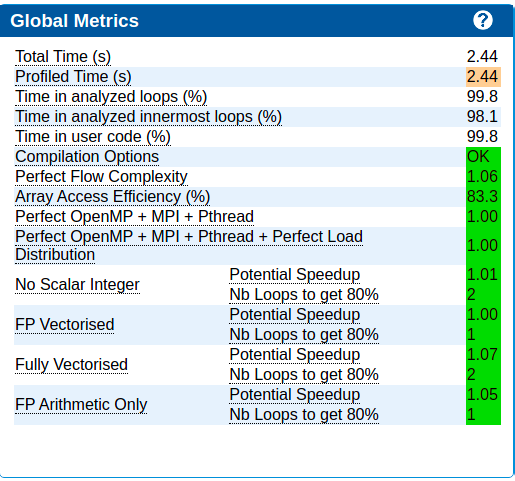
\includegraphics[scale=0.5]{Images/2/2-1.png}
    \caption{Global Metrics optimiser}
    \label{fig:my_label}
\end{figure}

\subsection{Application }
Meme dans l'application on remarque maintenant que le code s'éxecute à 99.79\% dans le code utilisateur.
\begin{figure}[H]
    \centering
    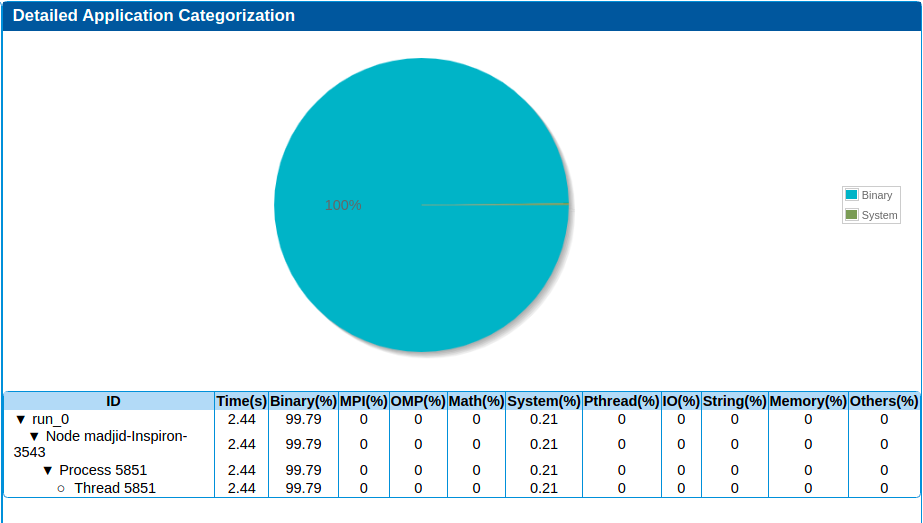
\includegraphics[scale=0.5]{Images/2/2-3.png}
    \caption{Application optimiser}
    \label{fig:my_label}
\end{figure}


\subsection{Loops}
\subsubsection{2.3.1 Loops Index}
Le code converge a 93\% et il s'est vectoriser a 61.05\%.
\begin{figure}[H]
    \centering
    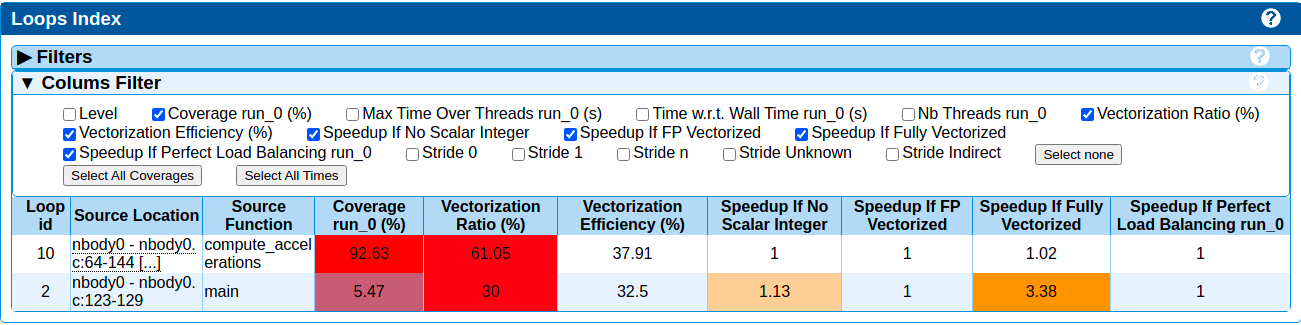
\includegraphics[scale=0.38]{Images/2/2-5.1.png}
    \caption{Hint}
    \label{fig:my_label}
\end{figure}


\end{document}


